%%%%%%%%%%%%%%%%%%%%%%%%%%%%%%%%%%%%%%%%%%%%%%%%%%%%%%%%%%%%%%%
%
% Welcome to Overleaf --- just edit your LaTeX on the left,
% and we'll compile it for you on the right. If you open the
% 'Share' menu, you can invite other users to edit at the same
% time. See www.overleaf.com/learn for more info. Enjoy!
%
%%%%%%%%%%%%%%%%%%%%%%%%%%%%%%%%%%%%%%%%%%%%%%%%%%%%%%%%%%%%%%%
\documentclass[border=2pt]{standalone}

% Drawing
\usepackage{tikz}
\usepackage{tikz-3dplot}

% Tikz Library
\usetikzlibrary{angles, quotes}

% Style
\tikzset{>=latex}

% Define Color
\definecolor{amber}{rgb}{1.0, 0.5, 0}
\definecolor{darkmagenta}{rgb}{0.55, 0.0, 0.55}
\definecolor{bleudefrance}{rgb}{0.19, 0.55, 0.91}

% Notation
\usepackage{physics}

% Newcommand
\newcommand{\midlabelline}[3]{
   \node (midlabel) at ($ (#1)!.5!(#2) $) {\huge #3};
   \draw[<-, very thick] (#1) --  (midlabel);
   \draw[->|, very thick] (midlabel) -- (#2);
}
\newcommand{\midlabellinee}[3]{
   \node (midlabel) at ($ (#1)!.5!(#2) $) {\huge #3};
   \draw[|<-, very thick] (#1) --  (midlabel);
   \draw[->|, very thick] (midlabel) -- (#2);
}

\newcommand{\midlabellineee}[3]{
   \node (midlabel) at ($ (#1)!.5!(#2) $) {\huge #3};
   \draw[very thick] (#1) --  (midlabel);
   \draw[very thick] (midlabel) -- (#2);
}

%Styles
%%Arrow in the Middle
\tikzset{midarrow/.style = {postaction=decorate, decoration={markings,mark=at position .52 with \arrow{stealth}}}}

% Define Length
\def\dy{0.45}

\begin{document}

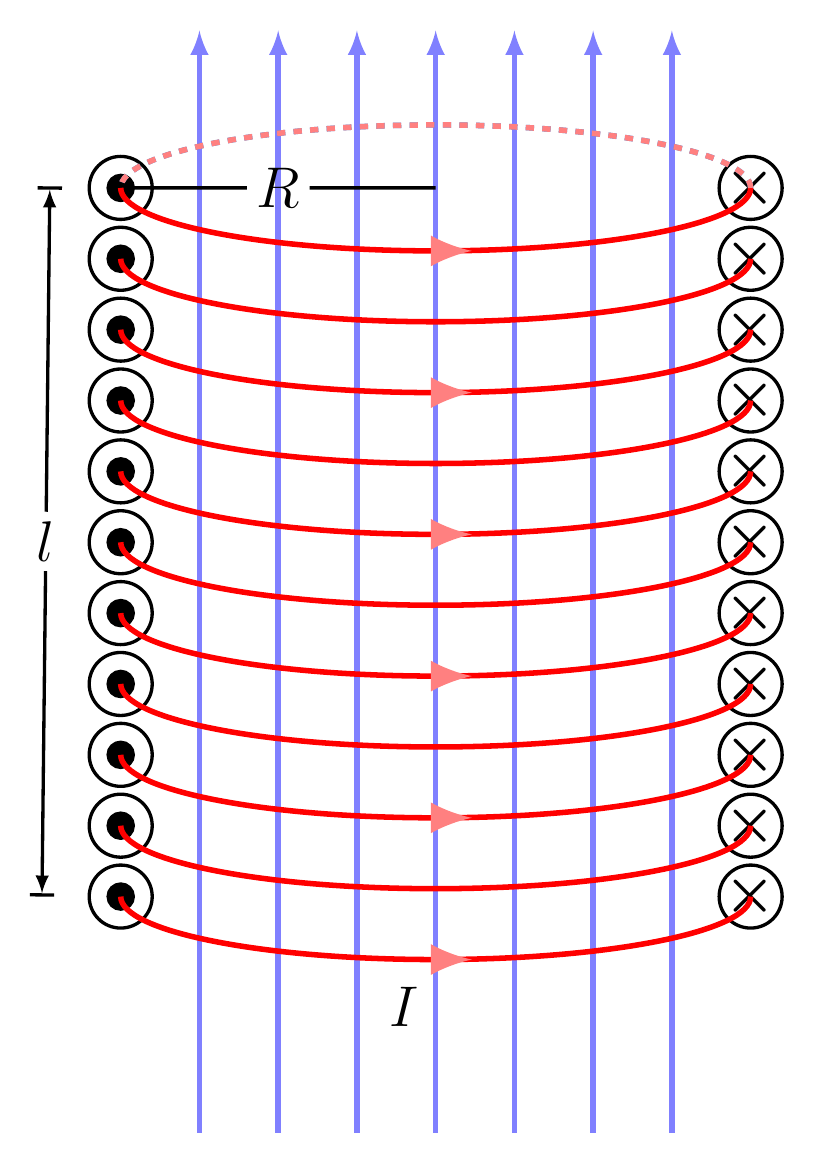
\begin{tikzpicture}[scale=2]
	% Grid
%	\draw[help lines] (0,0) grid (13,13);

    \foreach \x in {4.5,5,...,7.5}{
        \draw[->, blue!50, line width=2pt] (\x, 3) -- ++(0, 7);
    }

	% Symbols of Field Direction
	%% Left
	\foreach \i in {0,1,2,...,10}
	{
		\draw[very thick] (4,9-\i*\dy) circle [radius=0.2];
		\filldraw[very thick] (4,9-\i*\dy) circle [radius=0.08];
	}
	%% Right
	\foreach \i in {0,1,2,...,10}
	{
		\draw[very thick] (8,9-\i*\dy) circle [radius=2mm];
		\node at (8,9-\i*\dy) {\huge$\cross$};
	}

	% Semi Circle Dashed
	\draw[dashed, bleudefrance, line width = 2] (8,9) arc (0:180: 2 and 0.4);


	% Label Distances
	\midlabellinee{3.5,4.5}{3.55,9.01}{$l$}

	\midlabellineee{6,9}{4,9}{\huge$R$}

	% Semi Circles
	\foreach \i in {0,1,2,...,10}
	{
		\draw[red, line width = 2] (4,9-\i*\dy) arc (180:360: 2 and 0.4);
	}

	\foreach \i in {0,1,2,...,5}
	{
		\draw[red!50, line width = 4, ->] (6.05,8.6-2*\i*\dy) -- (6.230,8.6-2*\i*\dy);
	}
	%% Dashed
	\draw[dashed, red!50, line width = 2] (8,9) arc (0:180: 2 and 0.4);

	% Node
	\node at (5.8,3.8) {\huge$I$};


\end{tikzpicture}

\end{document}